\chapter{DESAIN DAN PERANCANGAN}
    Pada bab ini dibahas mengenai analisis dan perancangan sistem.
	
    \section{Kasus Penggunaan}
    	Terdapat dua aktor dalam sistem ini, yaitu pengembang (administrator) dan \textit{end-user} (pengguna) dari aplikasi web yang dikelola oleh sistem. Diagram kasus penggunaan digambarkan pada Gambar \ref{usecase}.
        \begin{figure}[H]
			\centering
			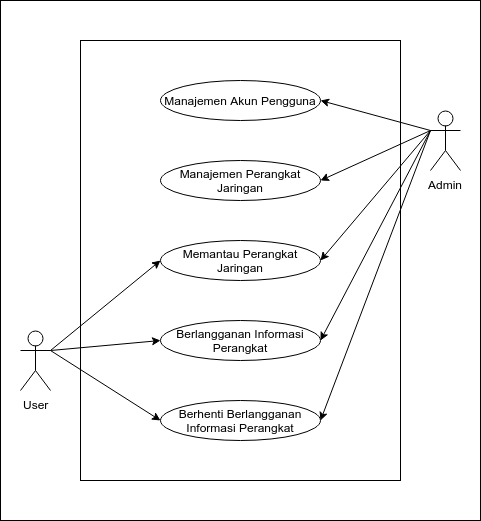
\includegraphics[width=8cm,height=10cm]{Images/C-3/usecase.png}
			\caption{Diagram Kasus Penggunaan}
			\label{usecase}
		\end{figure}
        \indent Diagram kasus penggunaan pada Gambar \ref{usecase} dideskripsikan masing-masing pada Tabel \ref {tabelKodeKasusPenggunaan}.
        
        \begin{longtable}{|p{0.25\textwidth}|p{0.24\textwidth}|p{0.35\textwidth}|} % L = Rata kiri untuk setiap kolom, | = garis batas vertikal.
		    	
		    	% Kepala tabel, berulang di setiap halaman
		    	\caption{Daftar Kode Kasus Penggunaan} \label{tabelKodeKasusPenggunaan} \\
		    	\hline
		    	\textbf{Kode Kasus Penggunaan} & \textbf{Nama Kasus Penggunaan} & \textbf{Keterangan} \\ \hline
		    	\endhead
		    	\endfoot
		    	\endlastfoot
		    	UC-0001 & Melihat daftar aplikasi \textit{web}. & Pengembang dapat melihat daftar aplikasi web yang ada di \textit{docker registry}. \\ \hline
		    	UC-0002 & Menjalankan aplikasi \textit{web}.  & Pengembang dapat menjalankan aplikasi web yang ada di \textit{docker registry} jika aplikasi dalam keadaan mati.\\ \hline
		    	UC-0003 & Mematikan aplikasi \textit{web}. & Pengembang dapat mematikan aplikasi web yang ada di \textit{docker registry} jika aplikasi sedang berjalan. \\ \hline
		    	UC-0004 & Mengganti port aplikasi \textit{web}. & Pengembang harus dapat mengganti port yang disediakan oleh aplikasi agar bisa diakses dari luar. \\ \hline
		    	UC-0005 & Melihat metrik sumber daya aplikasi \textit{web}. & Pengembang dapat melihat metrik dari sebuah aplikasi, yaitu jumlah \textit{container} dan jumlah request ke aplikasi. \\ \hline
                UC-0006 & Mengakses aplikasi yang sedang berjalan. & Pengembang dan \textit{end-user} dapat mengakses aplikasi yang sudah berjalan sesuai dengan domain yang diberikan oleh sistem. \\ \hline	
		    \end{longtable}

	\section{Arsitektur Sistem}
		Pada sub-bab ini, dibahas mengenai tahap analisis dan kebutuhan bisnis dan desain dari sistem yang akan dibangun.

		\subsection{Desain Umum Sistem}
			Sistem yang akan dibuat yaitu sistem yang dapat melakukan skalabilitas secara otomatis terhadap aplikasi web berbasis \textit{docker} dengan menggunakan \textit{Proactive Model} dan \textit{Reactive Model}.\\
			\indent Sistem ini akan digunakan oleh pengguna, yaitu \textit{end-user} dari aplikasi yang mana hanya bisa melakukan akses terhadap suatu aplikasi yang sudah berjalan. Selain itu juga digunakan oleh pengembang, yaitu orang mengelola aplikasi. Pengguna dari sistem ini hanya bisa melakukan akses atau permintaan kepada load balancer untuk mengakes aplikasi tertentu. Sedangkan pengembang dapat menambahkan dan memperbarui aplikasi web ke \textit{Private Docker Repository}. Sistem akan secara otomatis akan memperbarui aplikasinya sesuai dengan yang aplikasi terakhir yang dimasukkan oleh pengembang. Penjelasan secara umum arsitektur sistem akan diuraikan pada Gambar \ref{DesainUmumSistem}. Secara garis besar, ada empat \textit{server} yang akan digunakan membangun sistem ini, yaitu \textit{load balancer}, \textit{master host}, \textit{controller}, dan \textit{docker registry}.
            \begin{figure}[H]
				\centering
				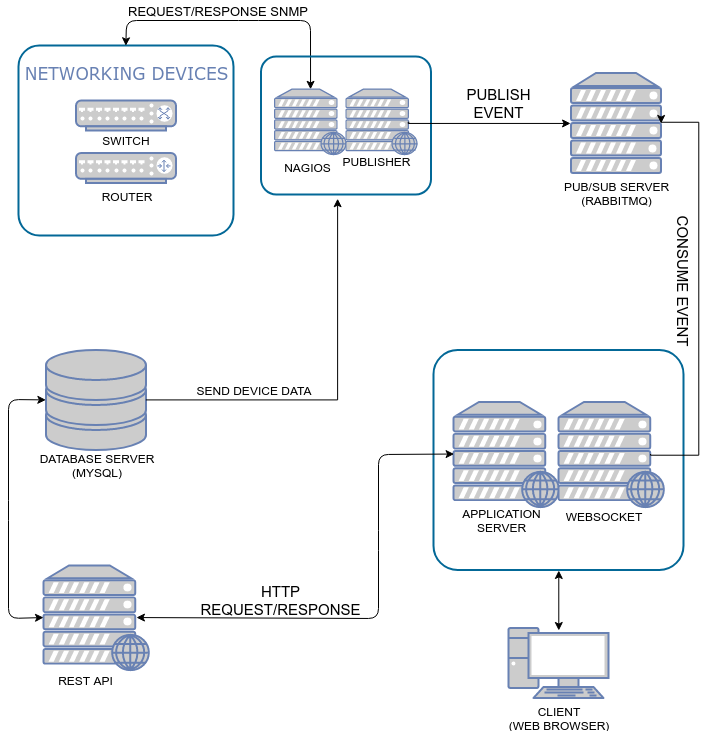
\includegraphics[width=9cm,height=8cm]{Images/C-3/main.png}
				\caption{Desain Umum Sistem}
				\label{DesainUmumSistem}
			\end{figure}

		\subsection{Desain Load Balancer}
            	\textit{Load balancer} digunakan sebagai pembagi beban aplikasi dan merekam permintaan dari pengguna. \textit{Load balancer} sendiri akan dibangun menggunakan perangkat lunak Haproxy.\\
                \indent Akses ke load balancer akan atur oleh DNS dari DigitalOcean. Pengguna bisa mengakses aplikasi web melalui domain yang disediakan. Saat melakukan akses domain, DNS DigialOcean akan mengarahkan permintaan ke server load balancer. Dari \textit{server load balancer}, HAProxy akan membaca domain mana yang diinginkan oleh pengguna. Setelah mengetahui domain yang dituju, HAProxy akan mengarahkan permintaan tersebut menuju \textit{container} dari aplikasinya. \\
            	\indent Haproxy akan menggunakan UNIX \textit{socket interface} sebagai perantara untuk mengelola log. Dengan memanfaatkan log tersebut, \textit{load balancer} menyediakan API tentang status dirinya yang dibutuhkan oleh \textit{server controller}. Log yang terdapat pada \textit{server} ini akan disajikan dengan memberikan sebuah \textit{endpoint}. \textit{Endpoint} akan dibangun dengan menggunakan kerangka kerja Flask. Secara umum, arsitektur dari \textit{server load balancer} dapat dilihat pada Gambar \ref{desain:loadbalancer}\\
                \begin{figure}[H]
                    \centering
                    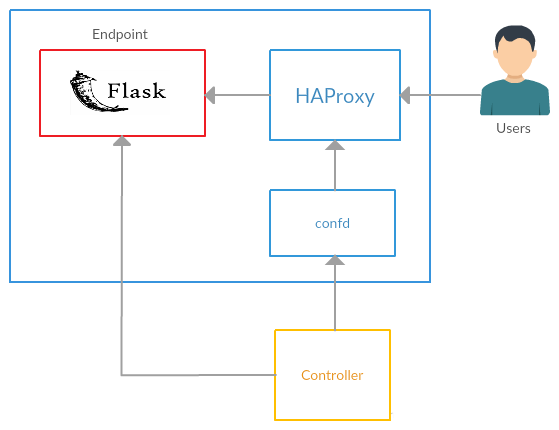
\includegraphics[width=7cm,height=7cm]{Images/C-3/loadbalancer.png}
                    \caption{Desain Load Balancer}
                    \label{desain:loadbalancer}
				\end{figure}
            	\indent Agar load balancer bisa mengetahui aplikasi yang sedang aktif, konfigurasi dari HAProxy akan dikelola oleh perangkat lunak bernama confd. Perangkat lunak ini akan membaca dari \textit{server controller} tentang konfigurasi yang paling baru. Jika terjadi perubahan data, maka confd akan menyesuaikan konfigurasi dari HAProxy agar sesuai dengan aplikasi yang tersedia. \\
            
		\subsection{Desain Private Docker Registry}
			\textit{Private docker registry}, yang selanjutnya hanya akan disebut \textit{docker registry}, digunakan untuk menyimpan \textit{docker image} aplikasi web yang dikelola oleh pengembang. \textit{Docker registry} akan dibangun di atas \textit{server} yang sudah memiliki \textit{docker engine} yang mana akan menjalankan dua \textit{container}, yaitu \textit{container docker registry} dan \textit{nginx}. \textit{Container docker registry} akan dibangun di atas \textit{image docker registry} yang secara resmi disediakan oleh Docker. Kemudian ada \textit{container} nginx yang akan digunakan untuk menghubungkan \textit{container docker registry} dengan jaringan luar. \textit{Nginx} digunakan agar \textit{container docker registry} bisa terlindungi dengan memanfaatkan fitur \textit{auth} yang dimilikinya. Selain itu juga proses pengaturan SSL dan domain relatif lebih mudah dan banyak referensi yang bisa digunakan dibandingkan dengan langsung memasangnya pada \textit{container docker registry}. Untuk membangun rancangan sistem tersebut, menggunakan \textit{docker compose}, yaitu sebuah perangkat lunak yang digunakan untuk mendesain rancangan sistem yang menggunakan \textit{docker} sebagai basisnya dan mengelola \textit{container} yang berjalan. Rancangan umum dari \textit{docker registry} seperti yang digambarkan pada Gambar \ref{desain:dockerregistry}.\\
            \indent Untuk menambah pengamanan dari \textit{docker registry} ini, aksessnya akan melalui protokol HTTPS. SSL yang akan dipakai disediakan oleh Let's Encrypt, sebuah lembaga yang menyediakan SSL secara gratis kepada umum. Selain itu, untuk mempermudah akses ke \textit{docker registry}, akan disediakan URL yang bisa digunakan oleh pengembang, yaitu \texttt{https://registry.nota-no.life}.
			\begin{figure}[H]
				\centering
				\includegraphics[width=7cm,height=6cm]{Images/C-3/dockerregistry.png}
				\caption{Desain Docker Registry}
				\label{desain:dockerregistry}
			\end{figure}
                
		\subsection{Desain \textit{Server Controller}}
        	\textit{Server controller} akan digunakan untuk memantau keseluruhan sistem. Terdapat dua subsistem utama pada \textit{server} ini, yaitu bagian yang menangani \textit{endpoint} dan bagian yang melakukan \textit{monitoring} terhadap sistem. Secara umum, arsitektur rancangan dari \textit{server controller} dapat dilihat pada Gambar \ref{Controller}. \\
            \indent Teknologi yang akan digunakan pada \textit{server} ini yang pertama adalah Flask, untuk membuat \textit{endpoint}. \textit{Endpoint} tersebut akan terhubung dengan MySQL, sebagai tempat penyimpanan data dari sistem, seperti data image pada \textit{docker registry}, \textit{container} yang sedang berjalan, dan domain yang didaftarkan pada DNS DigitalOcean. Lalu ada Redis, digunakan sebagai \textit{task queue} untuk pemrosesan data yang diberikan oleh \textit{endpoint}. Lalu terakhir, \textit{endpoint} akan terhubung dengan etcd, sebagai wadah untuk menyimpan konfigurasi \textit{load balancer}. \\
            \indent Selanjutnya terdapat \textit{script monitoring} menggunakan bahasa pemrograman Python. Fungsinya adalah untuk mengolah data yang ada pada sistem, seperti data pada \textit{load balancer} dan \textit{master host}. \textit{Script} ini juga yang akan menentukan keputusan untuk menambahkan atau mengurangi sumber daya yang ada pada sistem.
        	\begin{figure}[H]
				\centering
				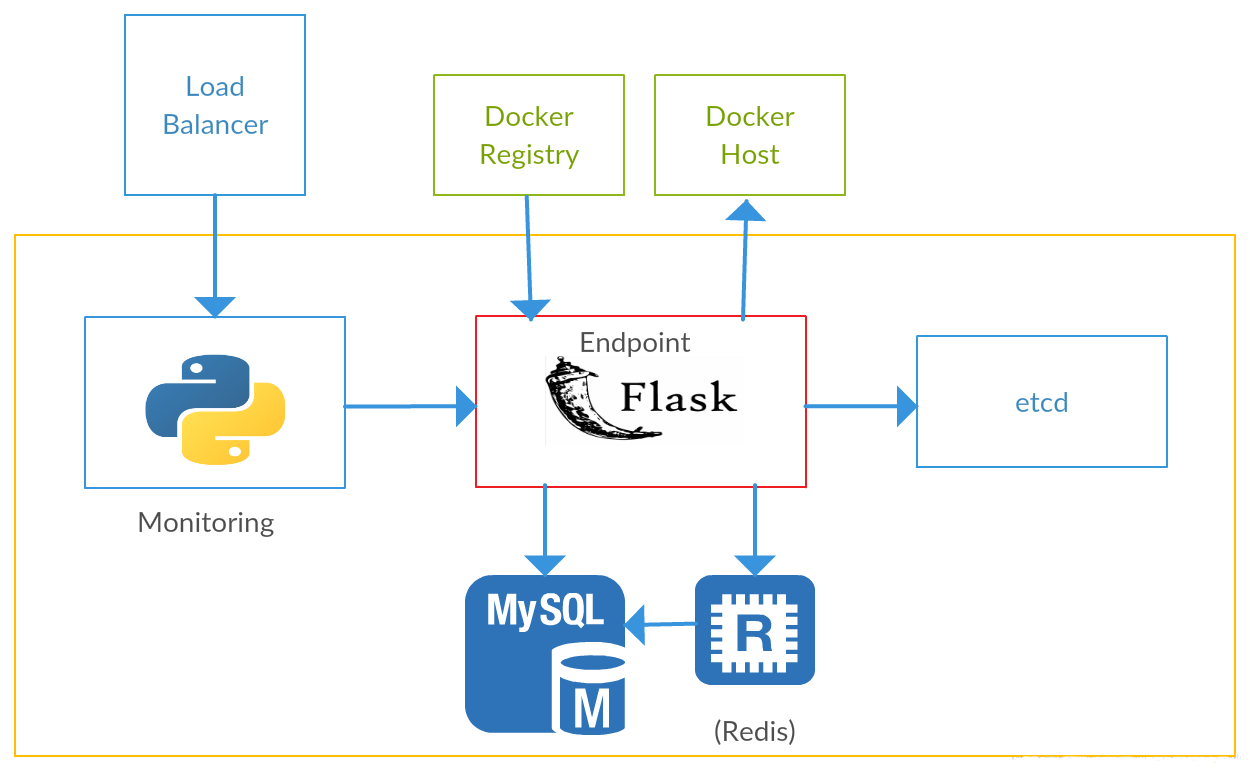
\includegraphics[width=8cm,height=7cm]{Images/C-3/controller.png}
				\caption{Desain Controller}
				\label{Controller}
			\end{figure}
            
            \subsubsection{Perancangan Endpoint}
            	\textit{Endpoint} yang dibuat di \textit{server} ini akan digunakan untuk berkomunikasi dengan \textit{host} lain. Pertama, terdapat sebuah \textit{endpoint} untuk menangkap notifikasi yang diberikan oleh \textit{docker registry} jika terjadi suatu kejadian. Penjelasan cara kerja dari \textit{endpoint} ini ditunjukkan pada Gambar \ref{endpointdockerregistry}. Selain itu juga disediakan \textit{endpoint} untuk kebutuhan dasbor, seperti untuk mendaftar aplikasi yang tersedia, informasi secara rinci dari aplikasi yang ada, dan status dari aplikasi.
            \begin{figure}[H]
				\centering
				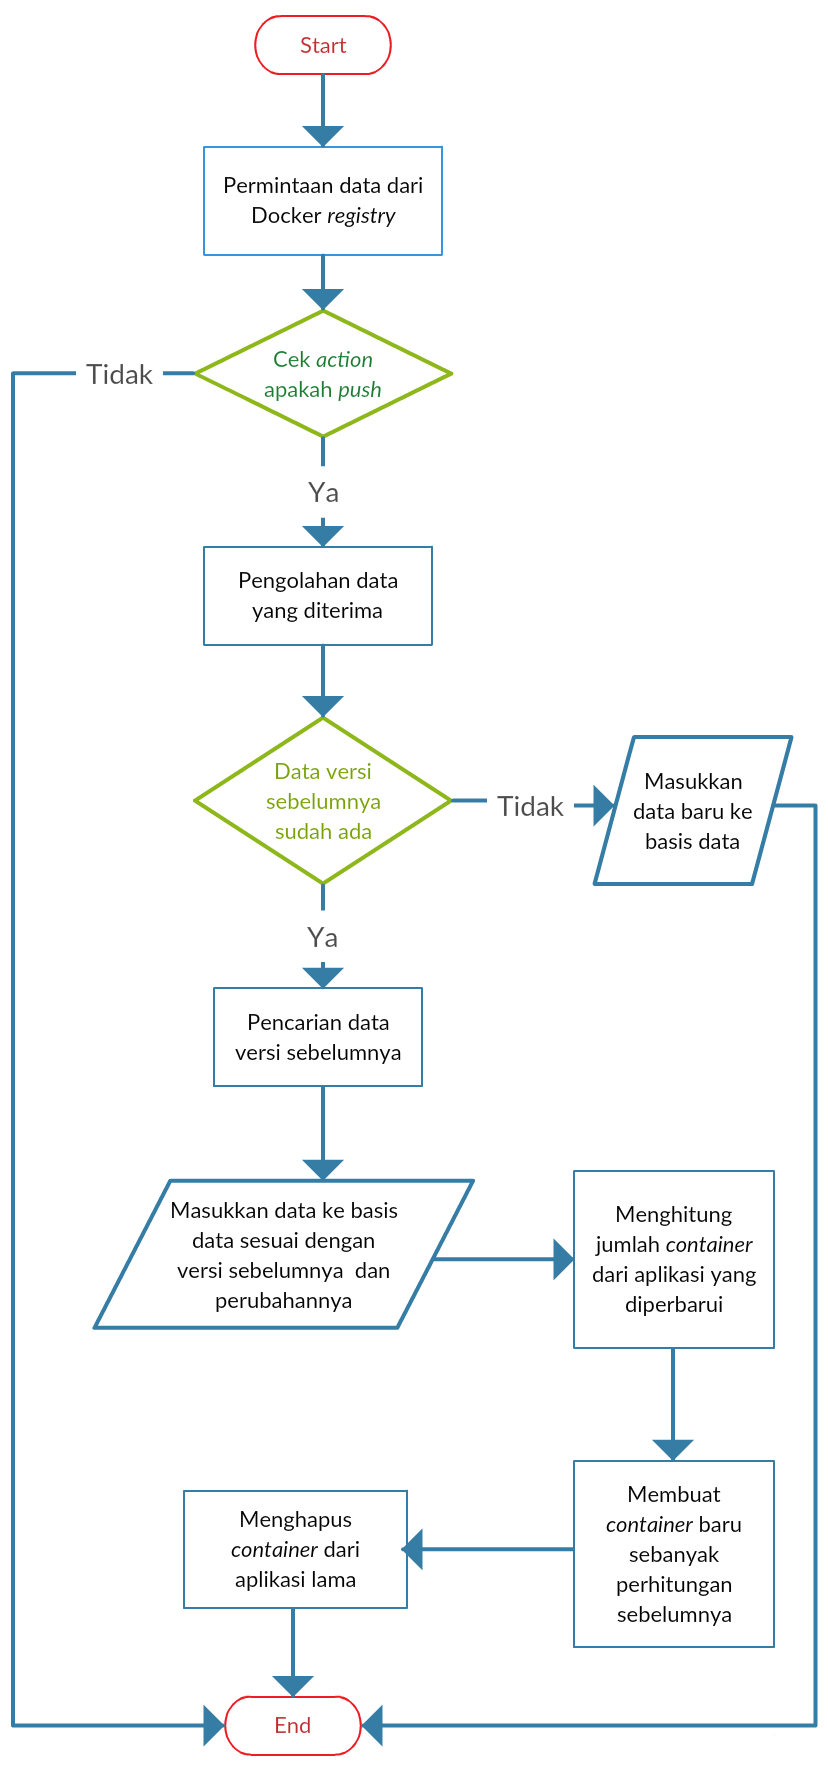
\includegraphics[width=7cm,height=15cm]{Images/C-3/endpointdockerregistry.png}
				\caption{Diagram Alur Pengelolaan \textit{Notification} Docker \textit{Registry}}
				\label{endpointdockerregistry}
			\end{figure}
                
            \subsubsection{Perancangan Sistem Monitoring}
            	Sistem monitoring merupakan subsistem yang ada \textit{server controller}. Sistem ini bertugas untuk mengolah data dan memantau sistem secara keseluruhan. Data yang akan diolah berasal dari \textit{master host} dan \textit{load balancer}. Dari \textit{server master host} akan didapatkan data penggunaan CPU dan \textit{memory} dari \textit{container} aplikasi-aplikasi yang sedang berjalan. Kemudian dari \textit{server load balancer} akan didapatkan data jumlah \textit{request} ke aplikasi. Dari data-data tersebut, proses perhitungan dengan menggunakan \textit{Proactive Model} dan \textit{Reactive Model} akan dilakukan. \\
                \indent \textit{Proactive Model} akan menggunakan data dari jumlah \textit{request} yang ada pada server \textit{load balancer} untuk melakukan prediksi berapa jumlah \textit{request} kedepannya dengan menggunakan perhitungan berdasarkan ARIMA. \\
                \indent \textit{Reactive Model} akan menggunakan data CPU dan \textit{memory} untuk menentukan apakah sumber daya dari aplikasi sudah melebihi batas yang ditentukan atau tidak. Jika sudah melebihi batas atas, maka akan ditentukan berapa jumlah \textit{container} yang diperlukan untuk mengatasi hal tersebut. \\
                \indent Dari perhitungan di atas, maka sistem ini akan melakukan penambahan atau pengurangan \textit{container} berdasarkan kebutuhan. Sistem ini akan memberitahu \textit{master host} untuk penyesuaian sumber daya dan juga melakukan pembaruan konfigurasi dari aplikasi. Pembaruan tersebut berguna agar \textit{server load balancer} bisa mengetahui keaadaan terbaru dari aplikasi dan \textit{container} yang berjalan di atasnya.
                
            \subsubsection{Penggunaan Task Queue}
            	Pada \textit{server controller} ini, akan banyak proses yang berjalan dalam jangka waktu yang panjang karena melakukan banyak eksekusi perintah di dalamnya. Jika proses tersebut berada di dalam fungsi yang dipanggil melalui protokol HTTP, maka umpan balik yang diberikan akan menunggu semua proses yang ada di dalamnya selesai. Hal tersebut akan membuat klien yang melakukan permintaan perlu menunggu dan merupakan hal yang tidak efisien. Untuk mengatasi hal tersebut, proses yang memerlukan banyak perintah, akan dimasukkan ke dalam sebuah \textit{queue} atau yang bisa disebut sebagai \textit{task queue}. Untuk task queue nya akan menggunakan Redis sebagai wadah untuk menampung perintah atau fungsi yang akan dikerjakan. Lalu, untuk menjalankan perintah atau fungsi yang sudah masuk ke dalam Redis, akan menggunakan \textit{worker} yang disediakan oleh pustaka Python bernama RQ.
            
		\subsection{Desain Master Host}
        	\begin{figure}[H]
				\centering
				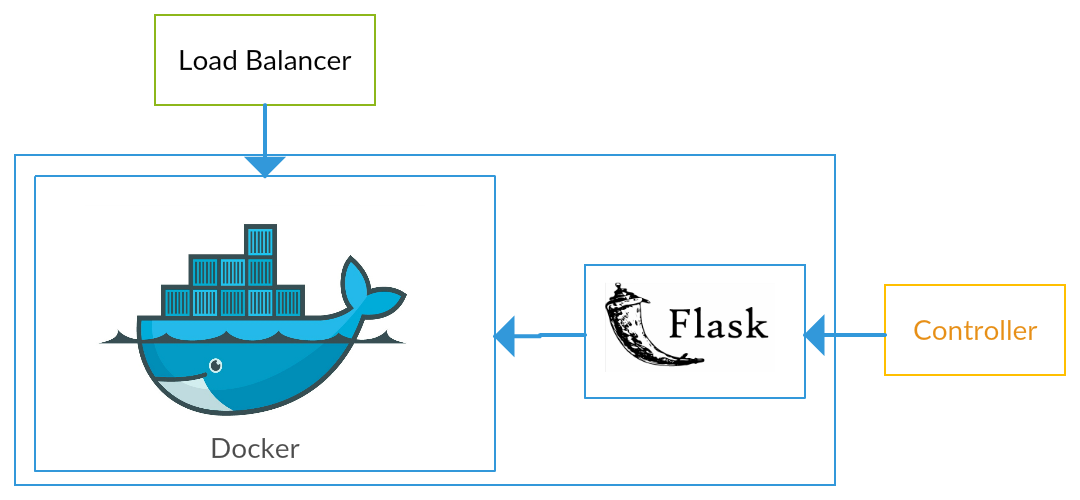
\includegraphics[width=8cm,height=5cm]{Images/C-3/masterhost.png}
				\caption{Desain Master Host}
				\label{desain:masterhost}
			\end{figure}
            \textit{Master host} merupakan sebuah \textit{server} yang akan menjalankan apalikasi-aplikasi yang diinginkan oleh pengembang. \textit{Host} ini memiliki \textit{docker engine} yang berguna untuk menjalankan \textit{container} dari aplikasi-aplikasi. Pada host ini akan dipasang \texttt{dockerpy} sebagai API untuk mengambil informasi-informasi dari \textit{container}, seperti penggunaan \textit{memory} dan CPU. Data-data digunakan oleh \textit{server controller} untuk mengetahui informasi \textit{container} yang ada dan juga digunakan untuk memberitahu \textit{host} apakah harus menambah atau mengurangi \textit{container} dari sebuah aplikasi. \textit{server controller} dapat mengakses data tersebut melalui layanan yang dibuat menggunakan perangkat kerja Flask. Dengan menggunakan perangkat kerja tersebut, layanan yang diberikan akan berjalan pada protokol HTTP. \\
            \begin{figure}[H]
				\centering
				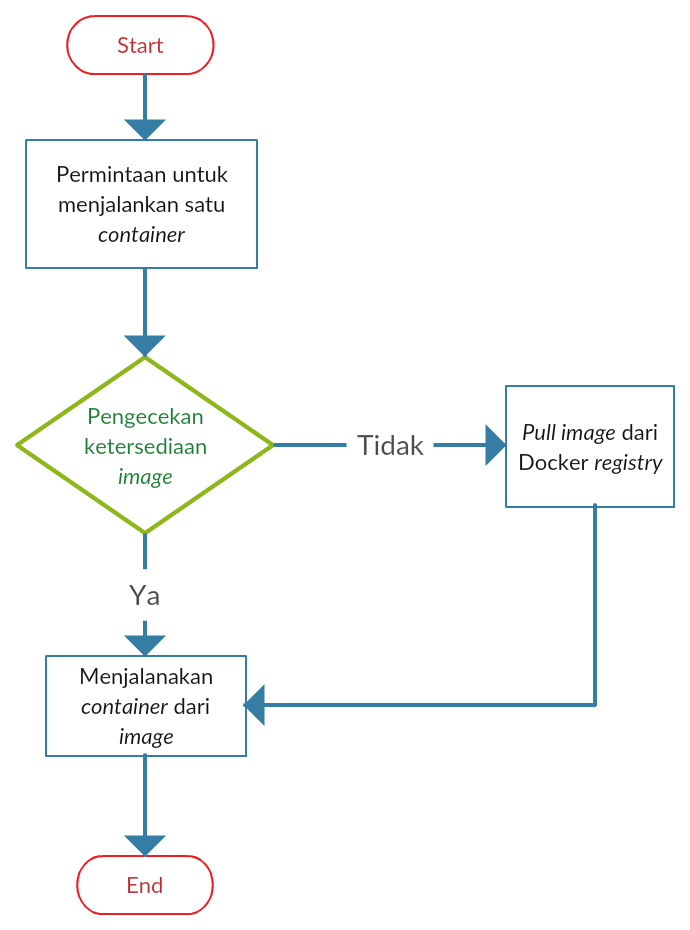
\includegraphics[width=7cm,height=10cm]{Images/C-3/createcontainer.png}
				\caption{Diagram Alur Menjalankan \textit{Container}}
				\label{createcontainer}
			\end{figure}
            \indent \textit{Host} akan mengambil data aplikasi yang berupa \textit{docker image} yang akan di jadikan \textit{container} dari \textit{docker registry}. Secara umum, perancangan dari sistem ini dapat dilihat pada Gambar \ref{desain:masterhost}. Proses untuk menambahkan \textit{container} baru, diagram alurnya dapat dilihat pada Gambar \ref{createcontainer}. Lalu, proses untuk menghapus \textit{container} yang sedang berjalan, diagram alurnya ditunjukkan pada Gambar \ref{deletecontainer}.
            \begin{figure}[H]
				\centering
				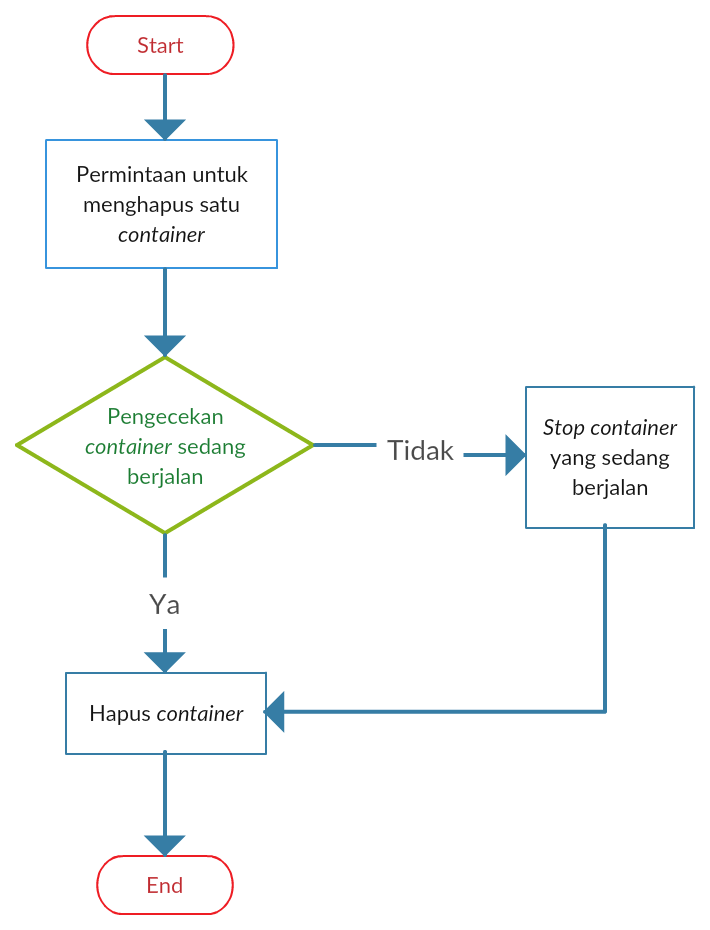
\includegraphics[width=6cm,height=10cm]{Images/C-3/deletecontainer.png}
				\caption{Diagram Alur Menghentikan \textit{Container}}
				\label{deletecontainer}
			\end{figure}
            \indent Terakhir, \textit{end-user} bisa melakukan akses terhadap aplikasi melewati \textit{load balancer}. \textit{Load balancer} yang akan mengarahkan pengguna untuk mengakses \textit{container} yang ada dari aplikasi.            
            
		\subsection{Desain Dasbor}
        	Dasbor adalah halaman yang digunakan sistem administrator untuk mengelola aplikasi dan menampilkan status metrik dari aplikasi. Dasbor adalah aplikasi berbasis web yang dibangun menggunakan React sebagai tampilan depan halaman (\textit{frontend}) dan Flask sebagai \textit{backend}. Secara umum, arsitektur dari dasbor seperti pada Gambar \ref{desain:dasbor}. \\
            \begin{figure}[H]
				\centering
				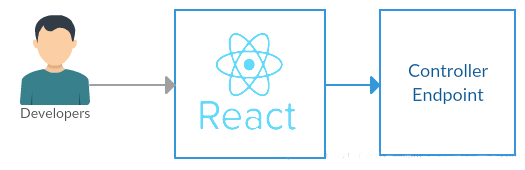
\includegraphics[width=8cm,height=3cm]{Images/C-3/dashboard.png}
				\caption{Desain Dasbor}
				\label{desain:dasbor}
			\end{figure}
            \indent Halaman depan akan menggunakan Material UI untuk mendapatan tampilan yang sederhana dan nyaman digunakan. Dasbor digunakan oleh sistem administrator untuk berinteraksi dengan sistem. Dasbor memiliki menu-menu yang memudahkan pengelolaan sistem. Menu-menu terdapat pada dasbor antara lain:
            \begin{itemize}
            \item Daftar Aplikasi \\
            	Halaman utama dari dasbor akan menampilkan daftar aplikasi yang ada pada \textit{docker registry}. Secara langsung, pengembang bisa langsung melihat status dari aplikasi, apakah sedang berjalan atau mati. Antar muka rancangannya ditunjukkan pada Gambar \ref{desain:dasborberanda}.
                
        	\begin{figure}[H]
				\centering
				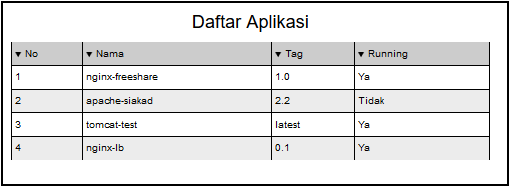
\includegraphics[width=9cm,height=4cm]{Images/C-3/beranda.png}
				\caption{Desain Antar Muka Dasbor Beranda}
				\label{desain:dasborberanda}
			\end{figure}
                
            \begin{figure}[H]
				\centering
				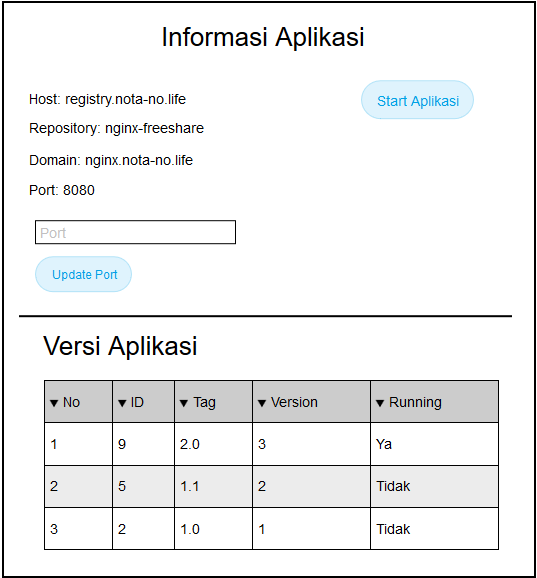
\includegraphics[width=9cm,height=9cm]{Images/C-3/image.png}
				\caption{Desain Antar Muka Informasi Aplikasi}
				\label{desain:dasborimage}
			\end{figure}
            
            \item Informasi Aplikasi \\
            	Jika pengembang memilih salah satu dari aplikasi yang ada pada beranda, maka akan diarahkan ke halaman informasi dari aplikasi. Pada halaman ini, pengembang dapat menentukan port dari aplikasi, menjalankan aplikasi, menghentikan aplikasi, dan melihat versi aplikasi sebelumnya. Rancangan antar muka untuk halaman ini seperti yang digambarkan pada Gambar \ref{desain:dasborimage}.
            \begin{figure}[H]
				\centering
				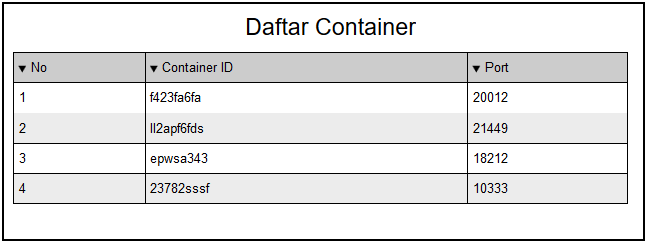
\includegraphics[width=8cm,height=5cm]{Images/C-3/container.png}
				\caption{Desain Antar Muka Daftar Container}
				\label{desain:dasborcontainer}
			\end{figure}
        
            \item Daftar Container \\
            	Pengembang juga disediakan halaman yang memperlihatkan data \textit{container} yang sedang berjalan dari suatu aplikasi. Pada data ini diinformasikan tentang ID dan port dari \textit{container} yang sedang berjalan. Antar muka untuk halaman ini seperti pada Gambar \ref{desain:dasborcontainer}.
            
            \item Metrik Aplikasi \\
            	Pada halaman ini, pengembang dapat melihat keadaan aplikasi, yaitu status jumlah akses dan jumlah \textit{container} pada waktu tersebut. Rancangan halaman ini ditunjukkan seperti pada Gambar \ref{desain:dasbormetrik}.
            \begin{figure}[H]
				\centering
				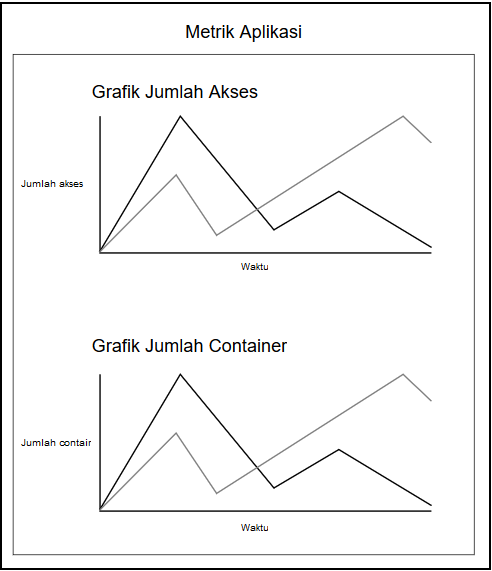
\includegraphics[width=8.3cm,height=9cm]{Images/C-3/metrik.png}
				\caption{Desain Antar Muka Metrik Aplikasi}
				\label{desain:dasbormetrik}
			\end{figure}
            \end{itemize}